%%%%%%%%%%%%%%%%%%%%%%%%%%%%%%%%%%%%%%%%%%%%%%%%%%%%%%%%%%%%%%%%%%%%%%
% Lớp 10 | Bất phương trình bậc 2 một ẩn | Giải bất phương trình bậc 2 một ẩn
% Dạng 0D7?2-1: Bất phương trình bậc 2 và ứng dụng
% Số câu: 28  (sinh tự động bởi tach_cau.py; từ nay thầy sửa trực tiếp file này)
%%%%%%%%%%%%%%%%%%%%%%%%%%%%%%%%%%%%%%%%%%%%%%%%%%%%%%%%%%%%%%%%%%%%%%

%%%%%%%%%%%%%%%% TRẮC NGHIỆM 4 PHƯƠNG ÁN %%%%%%%%%%%%%%%%

% nguồn: MaHoaNH_TracNghiem_Lop10
\begin{ex}%[0D7N2-1]%[ma:82e7fde5]
	Tập nghiệm của bất phương trình  $x^2+9> 6x$ là
	 \choice
		 {$(3;+\infty)$}
		{\True $\mathbb{R}  \setminus\{3\}$}
		{$\mathbb{R}$} 
		{$(-\infty; 3)$} 
	\loigiai{ 
	$x^2+9> 6x \Leftrightarrow(x-3)^2> 0\Leftrightarrow x \neq 3$.} 
\end{ex}

% nguồn: MaHoaNH_TracNghiem_Lop10
\begin{ex}%[0D7N2-1]%[ma:ffa6c463]
	Bất phương trình nào sau đây là bất phương  trình bậc hai một ẩn?
	\choice 
		{ $-3x+5y>1$} 
		{$x-7y-3z>2$} 
		{\True$2x^2+3x+1>0$} 
		{$2x^2-y>1$} 
	\loigiai{ 
		Bất phương trình bậc hai một  ẩn là $2x^2+3x+1>0$.
	 }
\end{ex}

% nguồn: MaHoaNH_TracNghiem_Lop10
\begin{ex}%[0D7N2-1]%[ma:933005c3]
	Tập  nghiệm của bất phương trình $x^2-5x+6\geq 0$ là
	\choice 
		 {\True $T=(-\infty;2]\cup[3;+\infty)$}
		{$T=(-\infty;1]\cup[6;+\infty)$} 
		 {$T=[2;3]$}
		{$T=[1;6]$} 
	 \loigiai{
		Bất phương trình $x^2-5x+6\geq 0$ có  tập nghiệm là $T=(-\infty;2]\cup[3;+\infty)$.
	 }
\end{ex}

% nguồn: MaHoaNH_TracNghiem_Lop10
\begin{ex}%[0D7N2-1]%[ma:ef72f623]
	Tập nghiệm của bất phương  trình $2x^2-14x+20<0$ là
	 \choice
		{$S=(-\infty; 2] \cup  [5;+\infty)$}
		{$S=(-\infty; 2) \cup  (5;+\infty)$}
		{\True $S=(2; 5)$} 
		{$S=[2;  5]$}
	\loigiai{ 
		 Ta có $2x^2-14x+20<0 \Leftrightarrow 2<x<5$.\\
		Vậy $S=(2;  5)$.
	 }
\end{ex}

% nguồn: MaHoaNH_TracNghiem_Lop10
\begin{ex}%[0D7N2-1]%[ma:4e5c76d7]
	Tập nghiệm của bất phương trình $x^2-x-6<  0$ có số nghiệm nguyên âm là
	 \choice
		 {$4$}
		 {$3$}
		{\True $1$} 
		 {$0$}
	 \loigiai{
		Ta có $x^2-x-6<  0\Leftrightarrow-2< x < 3$.\\
		Vậy nghiệm nghiệm âm của  bất phương trình là $x=-1$.
	} 
\end{ex}

% nguồn: MaHoaNH_TracNghiem_Lop10
\begin{ex}%[0D7N2-1]%[ma:d4fea2de]
	 Số nghiệm nguyên dương của bất phương trình $x^2-3 x-10<0$ là
	 \choice
		 {$3$}
		 {\True $4$}
		 {$-2<x<5$}
		{$6$} 
	\loigiai{ 
		 Ta có $x^2-3 x-10<0\Leftrightarrow -2<x<5$.\\
		Vì $ x  $ nguyên dương nên $ x\in \{1;2;3;4\} $.\\
		 Vậy bất phương trình có $ 4 $ nghiệm nguyên dương.
	 }
\end{ex}

% nguồn: MaHoaNH_TracNghiem_Lop10
\begin{ex}%[0D7N2-1]%[ma:f6c254eb]
	Tập nghiệm của bất phương trình $3x^2-2x-8  \leq 0$ chứa bao nhiêu số nguyên dương?
	\choice 
		{Vô  số}
		 {$0$}
		{$1$} 
		{\True $2$} 
	 \loigiai{
		Ta có $3x^2-2x-8=0 \Leftrightarrow \hoac{&x=2\\&x = -\dfrac{4}{3}.}$ 
		\begin{center}
			\begin{tikzpicture}[scale=1,font=\footnotesize,line join=round,line cap=round,>=stealth]
					\tkzTabInit[nocadre=false,lgt=3,espcl=2.5,deltacl=0.6] 
						{$x$/1,$3x^2-2x-8$/1} 
						{$-\infty$,$-\dfrac{4}{3}$,$2$,$+\infty$} 
					\tkzTabLine{,+,0,-,0,+,} 
				\end{tikzpicture}
		\end{center}
		Suy ra tập nghiệm  của bất phương trình là $\left[-\dfrac{4}{3}; 2 \right]$ chứa $2$ số nguyên dương.
	 }
\end{ex}

% nguồn: MaHoaNH_TracNghiem_Lop10
\begin{ex}%[0D7N2-1]%[ma:35a96976]
	Tập nghiệm  của bất phương trình $1-x^2<0$ là
	\choice 
		{$(0;1)$} 
		{$(-1;0)$} 
		{$(-1;1)$} 
		{\True $(-\infty;-1)\cup  (1;+\infty)$}
	 \loigiai{
		Tam thức  bậc hai $f(x)=1-x^2$ có hệ số $a=-1<0$ và có hai nghiệm $x_1=1$ và $x_2=-1$ nên ta có bảng xét dấu
		\begin{center}
			\begin{tikzpicture}[>=stealth,scale=1]
					\tkzTabInit[lgt=2,espcl=2.7] 
						{$x$/0.7,$f (x)$/0.7} 
						{$-\infty$,$-1$,$1$,$+\infty$} 
					 \tkzTabLine{,-,0,+,0,-,}
				\end{tikzpicture}
		\end{center}
		Từ bảng xét dấu, ta được tập nghiệm của bất phương trình là $(-\infty;-1) \cup  (1;+\infty)$.
	 }
\end{ex}

% nguồn: MaHoaNH_TracNghiem_Lop10
\begin{ex}%[0D7N2-1]%[ma:ee71e9d4]
	Xét dấu tam thức $f(x)=-3x^2+2x+8$. Khẳng  định nào sau đây đúng?
	 \choice
		 {\True $f(x) \geq 0$ khi $x \in\left[-\dfrac{4}{3}; 2\right]$}
		{$f(x) \leq 0$ khi  $x \in\left(-\infty;-\dfrac{4}{3}\right) \cup[2;+\infty)$}
		{$f(x) \leq 0$ khi  $x \in\left(-\dfrac{4}{3}; 2\right)$}
		{$f(x) \geq 0$ khi $x \in\left(-\dfrac{4}{3};  2\right)$}
	\loigiai{ 
		Ta  có $-3x^2+2x+8=0\Leftrightarrow\hoac{&x=2\\
		&x=-\dfrac{4}{3}.}$\\ 
		Bảng xét dấu 
		\begin{center}
			\begin{tikzpicture}[scale=0.8,font=\footnotesize,line join=round,line cap=round,>=stealth]
					\tkzTabInit[lgt=3] 
						{$x$/1.5,$f (x)$/1} 
						 {$-\infty$,$-\dfrac{4}{3}$,$2$,$+\infty$}
					 \tkzTabLine{,-,0,+,0,-,}
				\end{tikzpicture}
		\end{center}
		Khẳng  định $f(x) \geq 0$ khi $x \in\left[-\dfrac{4}{3}; 2\right]$.\\
		$f(x) \leq 0$ khi  $x \in\left(-\infty;-\dfrac{4}{3}\right]\cup \left[2;+\infty \right) $.
	} 
\end{ex}

% nguồn: MaHoaNH_TracNghiem_Lop10
\begin{ex}%[0D7H2-1]%[ma:2d579be5]
	Tìm tập  nghiệm $S$ của bất phương trình $-2x^{2}-3x+2>0$?\\
	\choice 
		{$S=\left(-\infty;-\dfrac{1}{2}\right)\cup(2;+\infty)$} 
		{$S=(-\infty;-2)\cup\left(\dfrac{1}{2};+\infty\right)$} 
		{\True $S=\left(-2;\dfrac{1}{2}\right)$} 
		{$S=\left(-\dfrac{1}{2};2\right)$} 
	 \loigiai{
		Ta  có $-2x^{2}-3x+2>0\Leftrightarrow-2<x<\dfrac{1}{2}$.\\
	} 
\end{ex}

% nguồn: MaHoaNH_TracNghiem_Lop10
\begin{ex}%[0D7H2-1]%[ma:eb271511]
	Tập nghiệm của bất phương  trình $-x^2+5x-4<0$ là
	\choice 
		 {$[1;4]$}
		{\True $(-\infty;1)\cup  (4;+\infty)$}
		{$(-\infty;1]\cup [4;+\infty)$} 
		 {$(1;4)$}
	\loigiai{ Ta có $-x^2+5x-4<0\Leftrightarrow x<1\ \text{hoặc} \  x>4$.\\
		Tập nghiệm của bất phương trình đã cho  là $(-\infty;1)\cup (4;+\infty)$.
	 }
\end{ex}

% nguồn: MaHoaNH_TracNghiem_Lop10
\begin{ex}%[0D7H2-1]%[ma:c1e84d7d]
	Cho tam thức bậc hai $f(x)=x^2+mx+n$, $(m, \,n \in  \mathbb{R})$ có $\Delta<0$. Khẳng định nào sau đây đúng?
	 \choice
		{$f(x)=0 \Leftrightarrow  x=-\dfrac{m}{2}$}
		 {$f(x)<0, \forall x \in(0;+\infty)$}
		 {\True $f(x)>0, \forall x \in \mathbb{R}$}
		 {$f(x)<0, \forall x \in \mathbb{R}$}
	 \loigiai{
		Tam  thức bậc hai $f(x)=x^2+mx+n$, $(m, \,n \in \mathbb{R})$ có $a=1>0$, $\Delta<0$.\\
		Vậy $f(x)>0, \forall x \in \mathbb{R}$. 
	 }
\end{ex}

% nguồn: MaHoaNH_TracNghiem_Lop10
\begin{ex}%[0D7H2-1]%[ma:d27e5633]
	Bất phương trình $(x-1)\left(x^2-7x+6\right) \geq 0$ có tập  nghiệm $S$ là
	\choice 
		{$S=(-\infty;  1] \cup[6;+\infty)$}
		 {$S=[6;+\infty)$}
		 {$(6;+\infty)$}
		{\True $S=[6;+\infty)  \cup\{1\}$}
	\loigiai{ 
		$(x-1)\left(x^2-7x+6\right) \geq 0\Leftrightarrow(x-1)^2(x-6) \geq  0\Leftrightarrow\hoac{&x-1=0\\
		&x-6\geq 0} \Leftrightarrow\hoac{&x=1\\ 
	&x \geq  6.}$}
\end{ex}

% nguồn: MaHoaNH_TracNghiem_Lop10
\begin{ex}%[0D7H2-1]%[ma:2dd899a5]
	Cho bất phương trình $x^2+bx+c > 0$. Tìm tập nghiệm  $S$ của bất phương trình đó biết rằng $b^2-4c < 0$.
	 \choice
		{$S=\left\{-\dfrac{b}{2}  \right\}$}
		{$S={\bf \mathbb{R}}\setminus \left\{-\dfrac{b}{2} \right\}$} 
		{\True  $S={\bf \mathbb{R}}$}
		{$S=\varnothing$} 
	 \loigiai{
		Ta có $b^2-4c < 0\Rightarrow \heva{&{a=1>  0} \\
		&{\Delta < 0}}\Rightarrow x^2+bx+c > 0$, $\forall x\in {\bf \mathbb{R}}\Rightarrow  S={\bf \mathbb{R}}$.
	 }
\end{ex}

% nguồn: MaHoaNH_TracNghiem_Lop10
\begin{ex}%[0D7H2-1]%[ma:5ed144e6]
	 Tập xác định của hàm số $y=\sqrt{6-x-x^2}$ là
	 \choice
		{\True $\mathscr{D}=[-3;2]$} 
		 {$\mathscr{D}=(-\infty;-3]\cup[2;+\infty)$}
		{$\mathscr{D}=(-\infty;-3)\cup(2;+\infty)$} 
		 {$\mathscr{D}=[-2;3]$}
	\loigiai{ 
		Điều  kiện $6-x-x^2\ge 0$.\\
		 Bảng xét dấu
		\begin{center}
			\begin{tikzpicture}
					 \tkzTabInit[lgt=2,espcl=2.5,deltacl=0.6]
						{$x$/0.8,$6-x-x^2$/0.8}{$-\infty$,$-3$,$2$,$+\infty$} 
					 \tkzTabLine{,-,0,+,0,-,}
				\end{tikzpicture}
		\end{center}
		Vậy tập xác định của hàm số $y=\sqrt{6-x-x^2}$ là $\mathscr{D}=[-3;2]$. 
	 }
\end{ex}

% nguồn: MaHoaNH_TracNghiem_Lop10
\begin{ex}%[0D7H2-1]%[ma:ca0c7092]
	Tập nghiệm $S$ của bất phương trình $x^{2}+x-6\leq  0$ là
	 \choice
		{$S=(-\infty;-3)\cup(2;+\infty)$} 
		{$S=(-\infty;-3]\cup[2;+\infty)$} 
		{$S=[-2;3]$} 
		 {\True $S=[-3;2]$}
	 \loigiai{
		Ta  có $x^{2}+x-6=0\Leftrightarrow\hoac{&x=-3\\&x=3.}$\\
		Bảng xét dấu 
		\begin{center}
			\begin{tikzpicture}
					 \tkzTabInit[nocadre=true,lgt=2,espcl=2.5,deltacl=0.5]
						{$x$/0.7,$x^2+x-6$/0.7} 
						 {$-\infty$,$-3$,$2$,$+\infty$}
					\tkzTabLine{,+,$0$,-,$0$,+} 
				\end{tikzpicture}
		\end{center}
		Từ bảng xét dấu, ta có $x^{2}+x-6\leq 0\Leftrightarrow x\in[-3;2]$. 
	 }
\end{ex}

% nguồn: MaHoaNH_TracNghiem_Lop10
\begin{ex}%[0D7H2-1]%[ma:2d867e8c]
	Tìm tập nghiệm  của bất phương trình $3x^2+30x+75 \leq 0$.
	\choice 
		{$S=\mathbb{R}  \backslash\{-5\}$}
		 {$S=\mathbb{R}$}
		{\True $S=\{-5\}$} 
		 {$S=\varnothing$}
	 \loigiai{
		Đặt $f(x)=3x^2+30x+75;  3x^2+30x+75= 0\Leftrightarrow x=-5$.\\
		Bảng xét dấu của  $3x^2+30x+75$\\
		\begin{center}
			\begin{tikzpicture}
					 \tkzTabInit[nocadre=true,deltacl=0.5,espcl=2.5,lgt=2]
						{$x$/1,$f (x)$/1} 
						 {$-\infty$,$-5$,$+\infty$}
					\tkzTabLine{,+,0,+} 
				\end{tikzpicture}
		\end{center}
		Vậy tập nghiệm của bất  phương trình là $S=\{-5\}$.
	 }
\end{ex}

% nguồn: MaHoaNH_TracNghiem_Lop10
\begin{ex}%[0D7H2-1]%[ma:48113540]
	Tìm tập nghiệm $S$ của bất  phương trình $x^2-4x+4> 0$.
	\choice 
		{\True $S=\mathbb{R}\setminus\{2\}$} 
		 {$S=\mathbb{R}$}
		{$S=(2;+\infty)$} 
		{$S=\mathbb{R}\setminus\{-2\}$} 
	 \loigiai{
		Xét $f(x)=x^2-4x+4=0\Leftrightarrow  x=2$.\\
		 Bảng xét dấu của $f(x)$ như sau
		\begin{center}
			\begin{tikzpicture}
					\tkzTabInit[deltacl=0.5,espcl=2.5,lgt=2,nocadre=false] 
						 {$x$/0.6,$f (x)$/0.6}
						 {$-\infty$,$2$,$+\infty$}
					 \tkzTabLine{,+,0,+,}
				\end{tikzpicture}
		\end{center}
		Vậy tập nghiệm của bất phương trình  là $S=\mathbb{R}\setminus\{2\}$.
	} 
\end{ex}

% nguồn: MaHoaNH_TracNghiem_Lop10
\begin{ex}%[0D7H2-1]%[ma:7848b585]
	Tập nghiệm của  bất phương trình $x^2-x-6\le0$ là
	\choice 
		{\True $S=[-2;3]$} 
		 {$S=(-\infty;-2]\cup[3;+\infty)$}
		{$S=(-2;3)$} 
		 {$S=(-\infty;-2)\cup(3;+\infty)$}
	 \loigiai{
		Ta có $x^2-x-6=0\Leftrightarrow\hoac{&x=-2\\&x=3.}$\\ 
		Do $a=1>0$  nên bảng xét dấu của biểu thức vế trái như hình bên dưới
		\begin{center}
			\begin{tikzpicture}[scale=1,font=\footnotesize,line join=round,line cap=round,>=stealth]
					\tkzTabInit[nocadre=false,lgt=2,espcl=1.8,deltacl=0.6] 
						{$x$/0.7,$x^2-x-6$/1} 
						{$-\infty$,$-2$,$3$,$+\infty$} 
					 \tkzTabLine{,+,0,-,0,+,}
				\end{tikzpicture}
		\end{center}
		Từ bảng xét dấu, tập nghiệm bất phương  trình là $S=[-2;3]$.
	} 
\end{ex}


%%%%%%%%%%%%%%%% ĐÚNG/SAI %%%%%%%%%%%%%%%%

% nguồn: MaHoaNH_DungSai_Lop10
\begin{ex}%[0D7N2-1]%[ma:48a80d0e]
	Mỗi khẳng định dưới đây đúng hay  sai?
	 \choiceTF
		{\True $x^2+x-3\geq 0$ là bất phương trình bậc hai  ẩn $x$}
		{$x\left(2-x^3\right)<3-x^2-x^3$ không phải là bất phương  trình bậc hai ẩn $x$}
		{Bất phương trình bậc hai $2x^2-3x+1>0$ có một  nghiệm là $x=1$}
		{\True Bất phương trình bậc hai $3x^2+x-5<0$ có một nghiệm là $x=0$} 
	\loigiai{ 
		\begin{itemchoice}
			\itemch $x^2+x-3\geq 0$  là bất phương trình bậc hai ẩn $x$.
			\itemch Ta có $x\left(2-x^2\right)<3-x^2-x^3 \Leftrightarrow x^2+2x-3<0$. Suy ra bất phương trình đã cho là bất phương trình bậc  hai ẩn $x$.
			\itemch Ta có $2\cdot 1^2-3\cdot 1+1=0$ nên $x=1$ không phải là nghiệm của  bất phương trình bậc hai $2x^2-3x+1>0$.
			\itemch Ta có $3\cdot 0^2+0-5=-5<0$ nên $x=0$  là nghiệm của bất phương trình bậc hai $3x^2+x-5<0$.
		\end{itemchoice}
	 }
\end{ex}

% nguồn: MaHoaNH_DungSai_Lop10
\begin{ex}%[0D7H2-1]%[ma:d2720dec]
	Cho bất phương trình  bậc hai $-x^2+6x-9\geq 0$.
	\choiceTF 
		{Bất phương trình đã cho vô nghiệm} 
		{\True Bất phương trình đã cho  có nghiệm duy nhất là $x=3$}
		{Bất phương  trình đã cho có tập nghiệm là $\mathbb{R}$}
		{Bất phương trình đã cho có tập nghiệm là $S=\left(-\infty;3\right)\cup\left(3;+\infty\right)$} 
	 \loigiai{
		Tam thức bậc hai $f(x)=-x^2+6x-9$ có biệt thức $\Delta'=3^2-(-1)\cdot(-9)=0$  nên có nghiệm $x=3$.\\
		Tam thức bậc hai $f(x)=-x^2+6x-9$ có  hệ số $a=-1<0$ nên có bảng xét dấu như sau:
		\begin{center}
			\begin{tikzpicture}
					 \tkzTabInit[nocadre=false,lgt=1.2,espcl=2.5,deltacl=0.5]
						{$x$  /0.7,$f (x)$/0.7}
						{$-\infty$,$3$,$+\infty$} 
					 \tkzTabLine{,-,$0$,-,}
				\end{tikzpicture}
		\end{center}
		Từ  bảng xét dấu suy ra bất phương trình đã cho có tập nghiệm là $S=\{3\}$.
	} 
\end{ex}

% nguồn: MaHoaNH_DungSai_Lop10
\begin{ex}%[0D7H2-1]%[ma:c57303c8]
	\immini 
	{Cho hàm số bậc hai $f(x)=ax^2+bx+c$ với $a\ne  0$ có đồ thị như hình vẽ bên.
	 \choiceTF
		{Hàm số  đồng biến trên khoảng $(-2;-1)$}
		{Giá trị nhỏ nhất của  hàm số là $-1$}
		{\True $2a+b+c=3$.} 
		{\True $f(x)\leq  2$ với mọi $x\in [-3;1]$}}
		{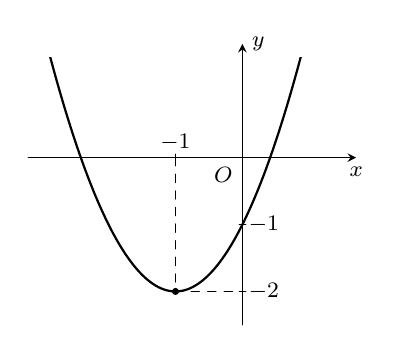
\begin{tikzpicture}[scale=0.85,line join=round,line cap=round,>=stealth,font=\footnotesize]
		\def\xmin{-3}\def\xmax{1.5}\def\ymin{-2.3}\def\ymax{1.5} 
		\draw[->] (\xmin-0.2,0)--(\xmax+0.2,0) node[below]{$x$}; 
		\draw[->] (0,\ymin-0.2)--(0,\ymax+0.2) node[right]{$y$}; 
		\draw (0,0) node[below left]{$O$}; 
		\draw (-1,0.05)--(-1,-0.05) node[above]{$-1$}; 
		\foreach \y  in {-2,-1}\draw (0.05,\y)--(-0.05,\y) node[right]{$\y$};
		\clip  (\xmin,\ymin) rectangle (\xmax,\ymax);
		\draw[thick,smooth,samples=200,domain=\xmin:\xmax]  plot (\x,{(\x)^2+2*(\x)-1});
		 \draw[dashed] (-1,0)--(-1,-2)--(0,-2); \fill (-1,-2) circle (1.5pt);
	\end{tikzpicture}
		 }
	 \loigiai{
		\begin{itemchoice}
			 \itemch Hàm số đồng biến trên khoảng $(-1;+\infty)$.
			\itemch Hàm số đạt giá trị nhỏ nhất bằng  $-2$ tại $x=-1$.
			\itemch Đồ thị hàm số đi qua $(0;-1)$ và có tọa độ đỉnh $(-1;-2)$  nên
			$$\heva{&c=-1\\& -\dfrac{b}{2a}=-1\\& a-b+c=-2} \Leftrightarrow \heva{&c=-1\\&2a-b=0\\&a-b+c=-2}  \Leftrightarrow \heva{&a=1\\&b=2\\&c=-1} \Rightarrow 2a+b+c=3 \Rightarrow f(x)=x^2+2x-1.$$
			\itemch Ta có $f(x)\leq 2 \Leftrightarrow  x^2+2x-1\leq 2 \Leftrightarrow x^2+2x-3\leq 0 \Leftrightarrow -3\leq x\leq 1$.
	\end{itemchoice}}
\end{ex}


%%%%%%%%%%%%%%%% TRẢ LỜI NGẮN %%%%%%%%%%%%%%%%

% nguồn: MaHoaNH_TraLoiNgan_Lop10
\begin{bt}%[0D7V2-1]%[ma:5f334ca8]
	Cho bất  phương trình $(m-1)x^2+2(m-1)x+1\le 0$. Có bao nhiêu giá trị nguyên của tham số $m$ để bất phương trình vô nghiệm?
	\shortans{1} 
	\loigiai{ 
		\textbf{Trường hợp 1:} $m-1=0\Leftrightarrow m = 1$.\\ Khi đó bất phương trình trở thành $1\le 0$ vô lý.\\Do đó $m=1$ bất  phương trình vô nghiệm. \\
		\textbf{Trường hợp 2:} $m-1\ne 0\Leftrightarrow m \ne 1$.\\ Khi đó $(m-1)x^2+2(m-1)x+1\le 0$ vô nghiệm khi và chỉ  khi
		$$\begin{aligned}
		& \ (m-1)x^2+2(m-1)x+1>0,\forall x \in \mathbb{R}  \\
		\Leftrightarrow & \ \heva{&m-1>0\\&(m-1)^2-(m-1)<0} \\ 
		\Leftrightarrow  & \ \heva{&m>1\\&1< m <2} \\
		\Leftrightarrow & \ 1< m  <2.
	\end{aligned}$$
	Vậy có 1 giá trị nguyên của $m$ thỏa mãn yêu  cầu bài toán.
 }
\end{bt}

% nguồn: MaHoaNH_TraLoiNgan_Lop10
\begin{bt}%[0D7V2-1]%[ma:e4db093a]
	Tập nghiệm của bất  phương trình $\left(x^2-x+6\right)^2-9\left(x^2-x\right)-46<0$ là khoảng $(a;b)$. Khi đó $b-a$ bằng bao nhiêu?
	\shortans{3} 
	 \loigiai{
	\textbf{Cách 1.}  \\
	Ta có 
	$$\begin{aligned}
	 & \ \left(x^2-x+6\right)^2-9\left(x^2-x\right)-46<0 \\
	\Leftrightarrow & \  \left(x^2-x\right)^2+3\left(x^2-x\right)-10<0 \\
	\Leftrightarrow & \ \heva{ & x^2-x>-5 \\ & x^2-x<2}  \\
	\Leftrightarrow & \ \heva{ & x^2-x+5>0 \ (\text{luôn đúng với mọi}  \ x\in\mathbb{R}) \\ & x^2-x-2<0} \\
	\Leftrightarrow & \  -1<x<2.
\end{aligned}$$
Do đó tập nghiệm  của bất phương trình đã cho là $(-1;2)$. \\
Vậy $a=-1$, $b=2$ và  $b-a=3$. \\
\textbf{Cách 2.} \\ 
Ta  có
$$\begin{aligned}
& \ \left(x^2-x+6\right)^2-9\left(x^2-x\right)-46<0 \\ 
\Leftrightarrow &  \ x^4+x^2+36-2x^3+12x^2-12x-9x^2+9x-46<0 \\
\Leftrightarrow  & \ x^4+4x^2-10-2x^3-3x<0 \\
\Leftrightarrow & \ x^4+x^3-3x^3-3x^2+7x^2+7x-10x-10<0 \\ 
\Leftrightarrow & \  \left(x^2-x-2\right)\left(x^2-x+5\right)<0 \\
\Leftrightarrow & \ x^2-x-2<0 \ (\text{vì} \ x^2-x+5>0, \forall  x\in\mathbb{R}) \\
 \Leftrightarrow & \ -1<x<2.
\end{aligned}$$
Do đó tập nghiệm của bất phương trình  đã cho là $(-1;2)$. \\
Vậy $a=-1$, $b=2$  và $b-a=3$.
 }
\end{bt}


%%%%%%%%%%%%%%%% TỰ LUẬN %%%%%%%%%%%%%%%%

% nguồn: MaHoaNH_TuLuan_Lop10
\begin{bt}%[0D7H2-1]%[ma:01c71277]
	Giải bất phương trình $x(x+5)\le 2(x^2+2)$. 
	 \loigiai{
		 Bất phương trình $x(x+5)\le 2(x^2+2)\Leftrightarrow x^2+5x\le 2x^2+4\Leftrightarrow x^2-5x+4\ge 0$.\\
		Xét phương trình $x^2-5x+4=0\Leftrightarrow \hoac{&x=1\\&x=4.}$\\ 
		 Lập bảng xét dấu
		\begin{center}
			\begin{tikzpicture}[scale=1,line join=round,line cap=round,>=stealth]
					\tkzTabInit[nocadre=false,lgt=4,espcl=2,deltacl=0.6] 
						{$x$  /0.6,$x^2-5x+4$ /0.6}
						{$-\infty$,$1$,$4$,$+\infty$} 
					\tkzTabLine{,+,0,-,0,+,} 
				\end{tikzpicture}
		\end{center}
		Dựa vào bảng xét  dấu, ta thấy $x^2-5x+4\ge 0\Leftrightarrow x\in (-\infty;1]\cup[4;+\infty)$.
	 }
\end{bt}

% nguồn: MaHoaNH_TuLuan_Lop10
\begin{bt}%[0D7K2-1]%[ma:c36605c9]
	Tìm$ m $để$ f(x)=x^2-2mx+m^2-m $luôn dương với mọi$ x $thuộc$ \mathbb{R}  $.
	\loigiai{$ f(x)=x^2-2mx+m^2-m $luôn dương với mọi$ x $thuộc$ \mathbb{R} $khi và chỉ khi 
		 $$\Delta' <0 \Leftrightarrow m^2-(m^2-m)<0\Leftrightarrow m<0.$$
		Vậy$ m<0 $thì$ f(x)=x^2-2mx+m^2-m $luôn dương với mọi$ x $thuộc$ \mathbb{R}  $.
	 }
\end{bt}

% nguồn: MaHoaNH_TuLuan_Lop10
\begin{bt}%[0D7B2-1]%[ma:281bee9c]
	Tìm $m$ để bất phương trình $x^2-2mx+3m+4>0,\,\forall x\in\mathbb{R}$ ($m$  là tham số).
	 \loigiai{
		Để bất phương trình $x^2-2mx+3m+4>0,\,\forall x\in\mathbb{R}$  thì
		 \allowdisplaybreaks
		\begin{eqnarray*}
			 &&\Delta'<0\\
			 &\Leftrightarrow&m^2-3m-4<0\\
			&\Leftrightarrow&-1<m<4. 
		\end{eqnarray*}
	} 
\end{bt}

% nguồn: MaHoaNH_TuLuan_Lop10
\begin{bt}%[0D7B2-1]%[ma:cdbfb714]
	Giải bất phương trình bậc hai sau  bằng cách lập bảng xét dấu:
	 \[3x^2-9x-30 \leq 4x(x-5).\]
	 \loigiai{
		Ta  có
		$$3x^2-9x-30 \leq 4x(x-5)  \Leftrightarrow -x^2+11x-30 \leq 0.$$
		Bảng xét  dấu
		\begin{center}
			\begin{tikzpicture}
					\tkzTabInit[lgt=4.5,espcl=3] 
						{$x$ /1,$-x^2+11x-30$  /1}
						{$-\infty$,$5$,$6$,$+\infty$} 
					\tkzTabLine{,-,0,+,0,-,} 
				\end{tikzpicture}
		\end{center}
		Vậy tập nghiệm của bất  phương trình đã cho là $S=(-\infty;5] \cup [6;+\infty)$.
	} 
\end{bt}
